% !TEX TS-program = xelatex
% !TEX encoding = UTF-8 Unicode
% !Mode:: "TeX:UTF-8"

%This file contains the LaTeX code of my laboratory report for my ICS II course.
%Author: 张作柏/Zuobai Zhang <17300240035@fudan.edu.cn>

% This is a simple template for a LaTeX document using the "article" class.
% See "book", "report", "letter" for other types of document.

\documentclass[12pt]{article} % use larger type; default would be 10pt

\usepackage[utf8]{inputenc} % set input encoding (not needed with XeLaTeX)

%%% Examples of Article customizations
% These packages are optional, depending whether you want the features they provide.
% See the LaTeX Companion or other references for full information.

%%% PAGE DIMENSIONS
\usepackage[top=1.05in, bottom=0.95in, left=0.90in, right=1.10in]{geometry}
%\usepackage{geometry} % to change the page dimensions
\geometry{a4paper} % or letterpaper (US) or a5paper or....
% \geometry{margin=2in} % for example, change the margins to 2 inches all round
% \geometry{landscape} % set up the page for landscape
%   read geometry.pdf for detailed page layout information

\usepackage{graphicx} % support the \includegraphics command and options

% \usepackage[parfill]{parskip} % Activate to begin paragraphs with an empty line rather than an indent

%%% PACKAGES
\usepackage{booktabs} % for much better looking tables
\usepackage{array} % for better arrays (eg matrices) in maths
\usepackage{paralist} % very flexible & customisable lists (eg. enumerate/itemize, etc.)
\usepackage{verbatim} % adds environment for commenting out blocks of text & for better verbatim
\usepackage{subfig} % make it possible to include more than one captioned figure/table in a single float
% These packages are all incorporated in the memoir class to one degree or another...

%%% HEADERS & FOOTERS
\usepackage{fancyhdr} % This should be set AFTER setting up the page geometry
\pagestyle{fancy} % options: empty , plain , fancy
%\renewcommand{\headrulewidth}{0pt} % customise the layout...
\lhead{}\chead{}\rhead{}
\lfoot{}\cfoot{\thepage}\rfoot{}

%%% SECTION TITLE APPEARANCE
\usepackage{sectsty}
\allsectionsfont{\sffamily\mdseries\upshape} % (See the fntguide.pdf for font help)
% (This matches ConTeXt defaults)

%%% ToC (table of contents) APPEARANCE
\usepackage[nottoc,notlof,notlot]{tocbibind} % Put the bibliography in the ToC
\usepackage[titles,subfigure]{tocloft} % Alter the style of the Table of Contents
\renewcommand{\cftsecfont}{\rmfamily\mdseries\upshape}
\renewcommand{\cftsecpagefont}{\rmfamily\mdseries\upshape} % No bold!
\usepackage{titletoc}
\titlecontents{section}
              [1.5cm]
              {\bf \large}%
              {\contentslabel{1.8em}}%
              {}%
              {\titlerule*[0.5pc]{$\cdot$}\contentspage\hspace*{0.6cm}}%
		   [\vspace{0.5em}]
\titlecontents{subsection}
              [1.8cm]
              {\normalsize}%
              {\contentslabel{2.0em}}%
              {}%
              {\titlerule*[0.5pc]{$\cdot$}\contentspage\hspace*{0.6cm}}%
		   [\vspace{0.4em}]
\titlecontents{subsubsection}
              [2.1cm]
              {\small}%
              {\contentslabel{2.5em}}%
              {}%
              {\titlerule*[0.5pc]{$\cdot$}\contentspage\hspace*{0.6cm}}%
		   [\vspace{0.4em}]


\usepackage[UTF8]{ctex}
\usepackage{fancyhdr}
\usepackage{enumerate}
\usepackage{indentfirst}
\usepackage{extramarks}
\usepackage{titling}
\usepackage{listings}
\usepackage{xcolor}
\usepackage{fontspec}
\usepackage[CJKbookmarks=true,colorlinks,linkcolor=black]{hyperref}
\setmainfont{Times New Roman}



\definecolor{mygreen}{rgb}{0,0.6,0}  
\definecolor{mygray}{rgb}{0.9,0.9,0.9}  
\definecolor{mymauve}{rgb}{0.58,0,0.82}  
  
\lstset{ %  
  backgroundcolor=\color{mygray},   % choose the background color; you must add \usepackage{color} or \usepackage{xcolor}  
  basicstyle=
	{
		\footnotesize
		\fontspec{Consolas}
	},        % the size of the fonts that are used for the code  
  breakatwhitespace=false,         % sets if automatic breaks should only happen at whitespace  
  breaklines=true,                 % sets automatic line breaking  
  captionpos=bl,                    % sets the caption-position to bottom  
  commentstyle=
	{
		\color{mygray}
		\fontspec{Consolas Italic}
	},    % comment style  
  deletekeywords={...},            % if you want to delete keywords from the given language  
  escapeinside={\%*}{*)},          % if you want to add LaTeX within your code  
  extendedchars=true,              % lets you use non-ASCII characters; for 8-bits encodings only, does not work with UTF-8  
  %frame=shadow,                    % adds a frame around the code  
  keepspaces=true,                 % keeps spaces in text, useful for keeping indentation of code (possibly needs columns=flexible)  
  keywordstyle=
	{
		\color{blue}
		\fontspec{Consolas Bold}
	},       % keyword style  
  %language=Python,                 % the language of the code  
  morekeywords={*,...},            % if you want to add more keywords to the set  
  numbers=none,                    % where to put the line-numbers; possible values are (none, left, right)  
  numbersep=5pt,                   % how far the line-numbers are from the code  
  numberstyle=\tiny\color{mygray}, % the style that is used for the line-numbers  
  rulecolor=\color{black},         % if not set, the frame-color may be changed on line-breaks within not-black text (e.g. comments (green here))  
  showspaces=false,                % show spaces everywhere adding particular underscores; it overrides 'showstringspaces'  
  showstringspaces=false,          % underline spaces within strings only  
  showtabs=false,                  % show tabs within strings adding particular underscores  
  stepnumber=1,                    % the step between two line-numbers. If it's 1, each line will be numbered  
  stringstyle=\color{blue},     % string literal style  
  tabsize=4,                       % sets default tabsize to 2 spaces  
  %title=myPython.py                   % show the filename of files included with \lstinputlisting; also try caption instead of title  
}  


%%% END Article customizations

%%% The "real" document content comes below...

%\title{\textbf{Digital Logic and Computer Design Report}}
\title{\textbf{MIPS多周期处理器实验报告}}
\author{张作柏\\17300240035}
%\date{} % Activate to display a given date or no date (if empty),
         % otherwise the current date is printed 

\begin{document}
\begin{sloppypar}
\maketitle

\pagestyle{fancy}
\lhead{\textbf{{\thetitle}}}
\rhead{\textbf{\nouppercase{\firstleftmark}}}
\cfoot{\thepage}

\thispagestyle{empty}
\tableofcontents
\clearpage

\setcounter{page}{1}

\section{多周期处理器简介}

单周期处理器虽然实现简单,但仍存在着许多问题。本节中,我们先简要讨论单周期处理器中的问题,借此引出多周期处理器,并介绍多周期处理器的主要特征。

\subsection{单周期处理器的缺点}

单周期处理器的主要缺点有三:
\begin{enumerate}
\item {\bf 效率低}:在单周期中,所有指令的执行时间都是一个CPU周期,这就意味着CPU周期的设置必须要保证所有指令都能在一个周期内执行完毕。而不同的指令执行效率是相差极大的,比如与访存相关的lw、sw指令所需要的时间远大于普通的R型运算指令。然而在实际系统中,用时较短的指令占到多数,为照顾耗时较长的指令而调高CPU周期是得不偿失的。

\item {\bf 资源浪费}:在单周期电路中,我们需要使用多个加法器,ALU和用于PC逻辑的多个加法器。那么,能否通过一个ALU就实现这些加法器的功能呢?虽然这样的节省在一个CPU上减少不了多少成本,但是当CPU进行批量生产时,则能省下较大的开支。

\item {\bf 内存设计不合理}:单周期处理器中,为了方便指令的执行,数据存储器与指令存储器是分离的。然而,在现实系统中往往二者是结合的。大多数计算机有一个单独的大容量存储器来存储指令和数据,并且支持读和写操作。
\end{enumerate}

\subsection{多周期处理器的特征}

多周期处理器通过将每个指令的执行过程分解为多个较短的步骤来解决这些问题。其主要特征为:
\begin{enumerate}
\item {\bf 状态机}:多周期将每条指令的执行分为多个阶段,每个阶段对应状态机中的一个状态。在这里使用状态机模型的好处是:1)合并不同指令执行中的公共状态 2)模式化状态转移的过程。因为不同指令的状态执行数不同,因此耗时也不同,用时较短的指令数量较少,可以大大减少其耗时。

\item {\bf 资源共享}:整个处理器只需要一个ALU,在多周期中,ALU利用闲置时间,充当原来多余加法器的角色,进行PC逻辑的计算。

\item {\bf 控制逻辑复杂}:因为引入了状态机模型,所以也就要考虑相应的状态转移,同时需要的控制逻辑也会变得更加复杂,带来更大的编程复杂度。同时,因为多周期的控制逻辑更加复杂,所以CPU也会在此花费更多的时间,最终导致多周期处理器的性能相对于单周期并不会带来非常大的提升。
\end{enumerate}

\newpage
\section{部件分析}

多周期处理器中大部分器件都与单周期相似,在此只列出新添加或发生改动的部件,其余请参考我的单周期报告。

\subsection{触发器flopr}

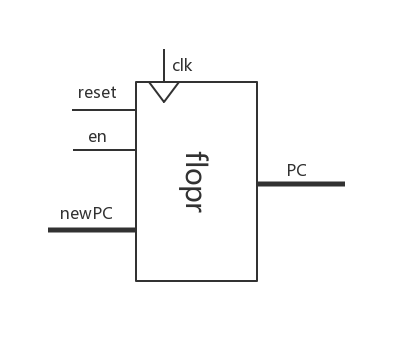
\includegraphics[width =0.35\linewidth]{figure/flopr.jpg}

多周期中的触发器增加了一个使能端口en,当时钟上升沿到达,若en=1,则将newPC写入PC,否则PC保持原值。增加这一端口的原因是,多周期中并不是每个上升沿都要进行写操作,有的寄存器需要保持原来存储的值不做变化。

\subsection{算数逻辑单元ALU}

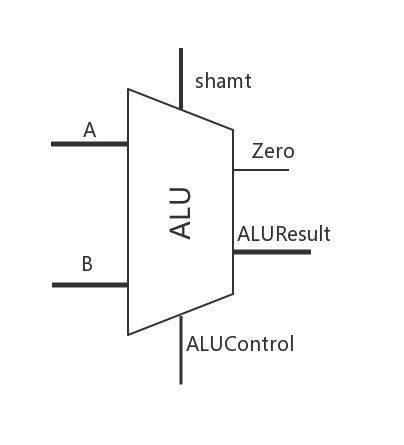
\includegraphics[width =0.3\linewidth]{figure/ALU.jpg}

按照原来的设计,其实单周期与多周期的ALU应该是相同的。然而,我现在在ALU上多加入了一个shamt口用来接收移位的数据,这样做的好处是减少了控制信号,同时也降低了控制的复杂度,随之而来的问题就是ALU的成本会变大。实际上,只有在移位操作时才会使用shamt,那么完全可以把shamt的数据通过A或B口传入,只不过会增加一些控制的难度罢了。

\subsection{存储器Mem}

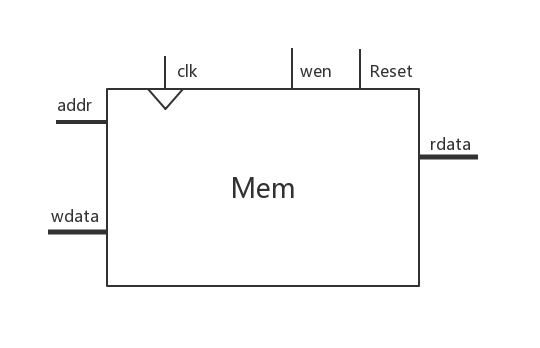
\includegraphics[width =0.4\linewidth]{figure/mem.jpg}

存储器最大的不同是将指令存储器Imem与数据存储器Dmem合并起来,以模拟真实情景。mem内部的构造与单周期的Dmem相同,只不过使用0~99的地址空间来存储指令,之后的地址空间才存储数据罢了。

\subsection{乘法器mul}

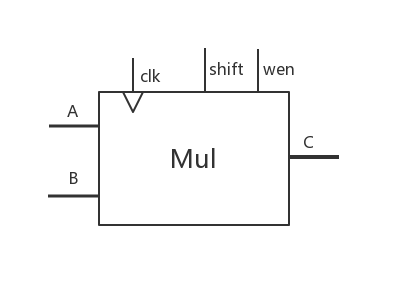
\includegraphics[width =0.4\linewidth]{figure/mul.jpg}

乘法器是新加入的部件,其功能是执行A与B的乘法,并将结果输出到C中,其中A与B都是四位二进制数,C是八位二进制数。在后面乘法器的原理分析中,我们可以发现可以很容易的将四位乘法拓展到32位乘法,在此为节省演示时间,只涉及了四位乘法的乘法器。

乘法器原理就是在计算机组成课上讲的移位乘法,利用一个8位寄存器存储当前结果,每次做加法写入高位后,将整个寄存器右移一位,四次移位后,即为答案。在实现的时候,我使用了shift和wen两个接口来接受控制器传来的移位信号与写使能信号:当wen信号为1时,将B的值写入结果寄存器低位,并将高位置为0;否则当shift信号为1,执行加法并左移操作;否则结果寄存器保持原值。这里我为乘法器模块单独设计了一个加法器,而实际上这里共用ALU是更划算的,然而控制逻辑有点复杂,所以我就偷了个懒。。。

\subsection{数据通路Datapath}
\noindent
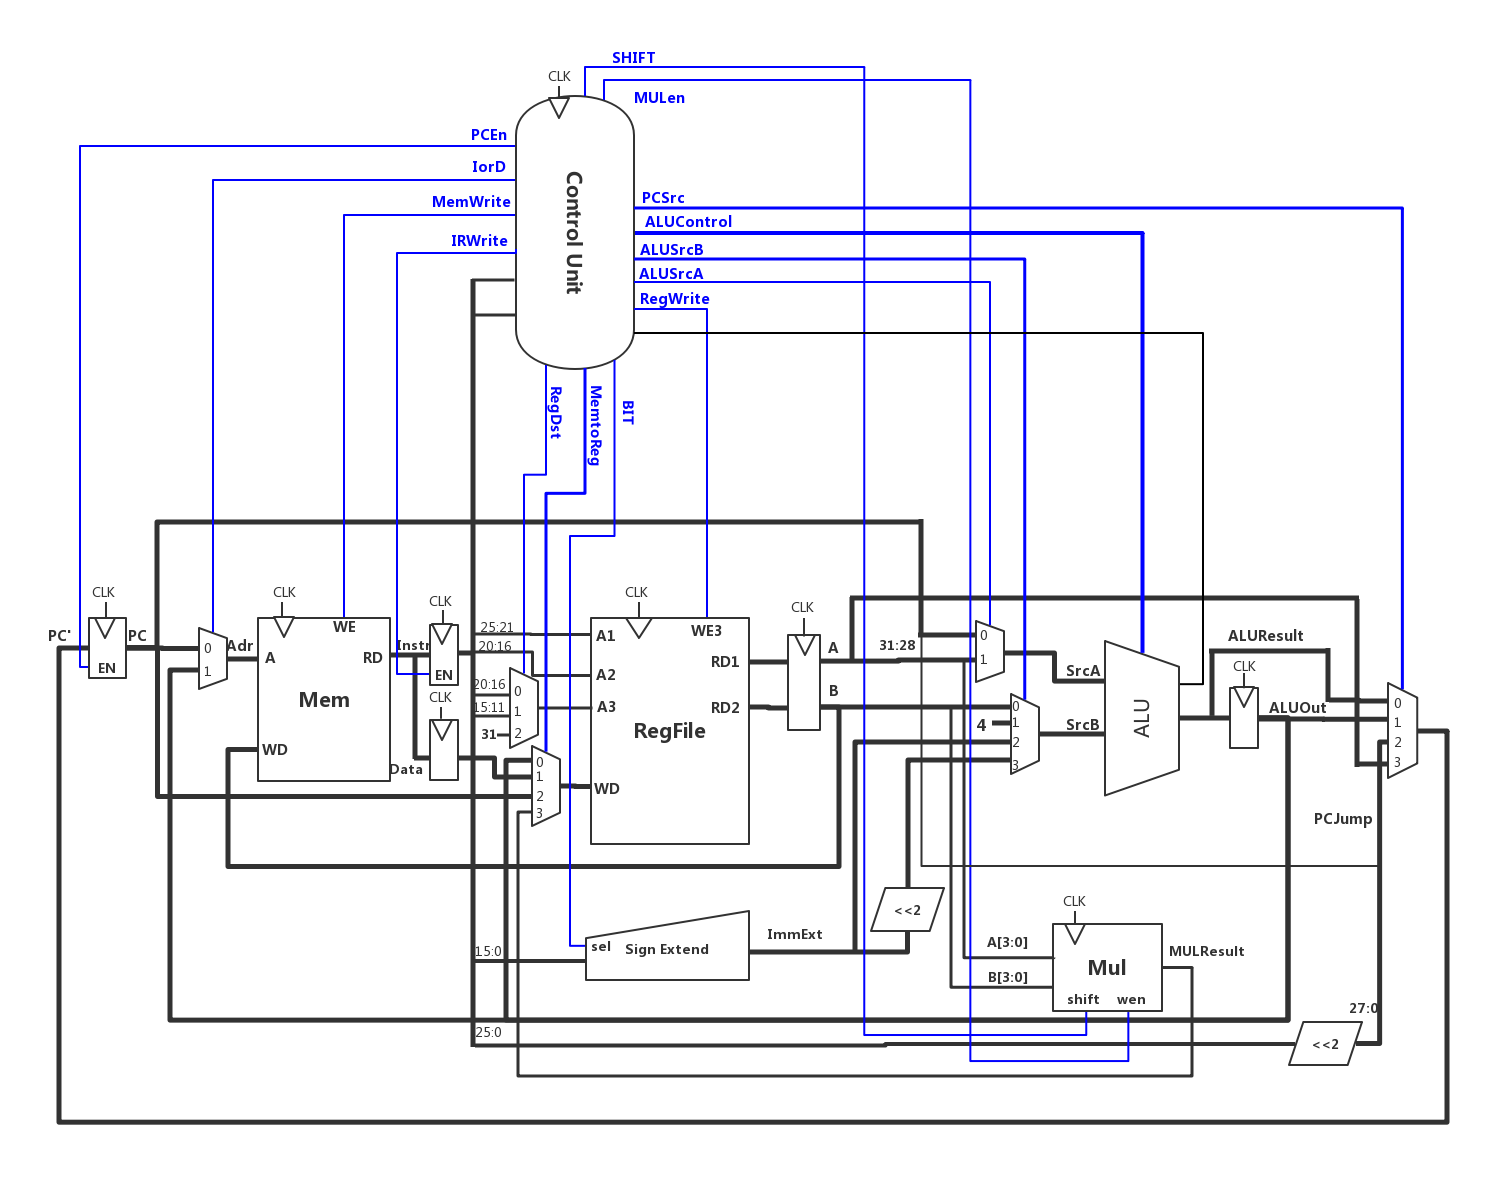
\includegraphics[width =\linewidth]{figure/Datapath.jpg}

{\bf 功能说明}:因为与单周期相比很多部件都没有改变,所以这里只说明变化的部分。
\begin{itemize}
\item 左侧PC寄存器,添加了PCEn信号,控制寄存器写入逻辑,只在需要更新PC值的状态才将PCEn设置为1。
\item 左侧二路选择器,因为Dmem与Imem合二为一了,所以要通过IorD信号选择读取指令还是读取数据。
\item 左侧Instr寄存器,只有当需要读指令时,才将IRWrite信号设为1,其余状态则需要存储原先的指令。
\item 中间A、B两个寄存器用于存从RegFile中读出来的值,因为这些值可能会延迟一个状态使用,所以需要用寄存器储存。
\item 中间SrcA是ALU的A参数,由ALUSrcA信号控制:当ALUSrcA为0时,选择PC值作为运算对象(常用作计算下一指令的PC值);当ALUSrcB为1时,选择A寄存器的值作为运算对象,用于R型和部分I型指令。
\item 中间SrcB是ALU的B参数,由ALUSrcB信号控制:当ALUSrcB为00时,选择B寄存器的值作为运算对象,用于R型指令;当ALUSrcB为01时,选择4作为运算对象,用于计算下一条指令的PC;当ALUSrcB为10时,选择移位前的立即数作为运算对象,用于I型指令;当ALUSrcB为11时,选择移位后的立即数作为运算对象,用于计算jal、bne、beq指令跳转的目标地址。
\item 右侧ALUOut寄存器用于存储ALU运算的结果,以供下一周期使用。
\item 右侧四路选择器用于选择PC的值,由PCSrc信号控制,共四种选择:ALUResult(下一指令PC),ALUOut(jal、bne、beq指令的跳转地址)、PCJump(j指令的跳转地址)、A(jr指令的跳转地址)。
\end{itemize}

\subsection{控制模块Controller}

\subsubsection{控制信号说明}

以下简单解释一下我使用的控制信号。
\begin{itemize}
\item PCEn用于控制是否写入PC,由PCWrite、Branch、Branch1和Zero信号控制:
\begin{lstlisting}[language=Verilog]  
assign PCEn = (Branch & Zero) | (BranchBNE & ~Zero) | PCWrite;
\end{lstlisting}  
\item IorD用于控制读指令还是数据
\item MemWrite用于控制是否写入内存
\item IRWrite用于控制是否将从Mem中读出的数据写入Instr寄存器
\item RegDst用于控制写入寄存器的选择
\item MemtoReg用于控制写入数据的来源
\item BIT用于控制移位是符号扩展还是0扩展
\item SHIFT和MULen分别作为乘法器的移位信号和写使能,将在乘法指令的实现细节中讨论
\item PCSrc用于选择PC值的来源
\item ALUControl用于控制ALU的运算
\item ALUSrcA、ALUSrcB用于选择ALU的A、B参数
\item RegWrite用于控制RegFile的写使能
\end{itemize}

\subsubsection{实现细节}

在单周期中,我们可以直接根据指令的类型来调整控制信号;而在多周期中,我们则需要根据当前所处的状态来进行信号赋值:
\begin{lstlisting}[language=Verilog]  
reg [21:0] controls;
    assign {SHIFT, MULen, IorD, memwrite, IRWrite, RegDst, MemtoReg, PCWrite, branch, branchBNE, ALUSrcA, RegWrite, BIT, ALUSrcB, PCSrc, aluop} = controls;   
    always @(*)
      case (state)
        Fetch        : controls <= 22'b0000100001000000100000;
        Decode       : controls <= 22'b0000000000000001100000;
	   ......
        default: controls <= 22'bx;
      endcase
\end{lstlisting}  

比单周期更复杂的是,多周期中增加了状态机的设置,也就需要我们书写状态机的转移代码。为了表示方便,我们可以先用易于理解的常量表示状态和指令:
\begin{lstlisting}[language=Verilog]  
parameter Fetch = 0;
parameter Decode = 1;
......
parameter LW = 6'b100011;
parameter SW = 6'b101011;
......
\end{lstlisting}  

之后,根据当前状态和指令的值,用case语句选择下一状态:
\begin{lstlisting}[language=Verilog]  
always @(*)
      case (state)
        Fetch: nextstate = Decode;
        Decode: case (op)
                  ......
                endcase
        MemAdr: case (op)
                  ......
                endcase
        MemRead: nextstate = MemWriteback;
        MemWriteback: nextstate = Fetch;
        ......
	  default: nextstate = 5'bx;
     endcase
\end{lstlisting}  

最后,在每个时钟上升沿到来时,用nextstate更新state:
\begin{lstlisting}[language=Verilog]  
always @(posedge clk or posedge Reset)
    if (Reset) state <= 0;
    else state = nextstate;
\end{lstlisting}  

\newpage
\section{有限状态机与指令分析}

\subsection{状态机图与状态分析}
\noindent
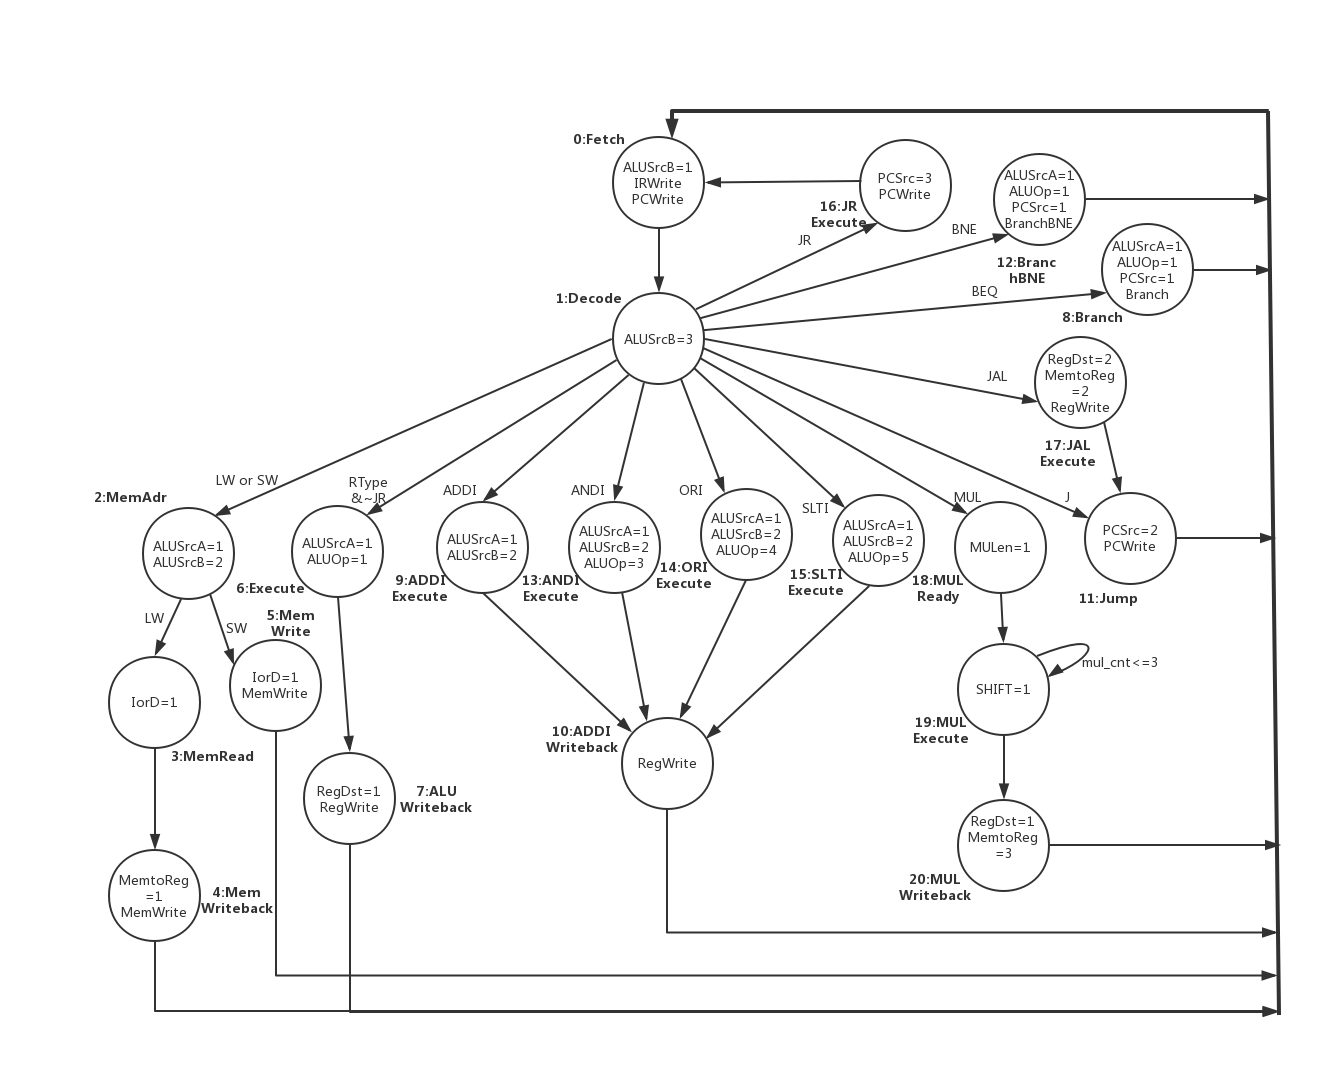
\includegraphics[width =\linewidth]{figure/State.jpg}

图中未标出的控制变量均默认为0。

\subsection{额外指令分析}

常规指令的状态设计在教材中已经分析的相当透彻了,因此我在这里只列出我增加的指令的状态设计思路。

\subsubsection{移位指令sll}

注意到,这里没有为移位指令单独设计状态,而是将其作为普通的R-Type指令来处理。因为我改造了ALU,把移位数传到了ALU中,这样就ALU就可以直接根据funct进行移位操作了。过程与其它R-Type指令完全一样,无需增加新的状态。

\subsubsection{函数调用指令jal}

我为jal指令新增加了一个状态17:JALExecute,在这个状态中我们要将返回地址写入寄存器\$ra中。那么,

之后,我们可以像jump一样,根据指令中的立即数计算目标地址,选择PCSrc为2,更新PC。

\subsubsection{跳转寄存器指令jr}

跳转寄存器指令也比较好实现,只需要为PC的来源增加一个选项为寄存器值即可。然后增加一个状态JRExecute,选择PCSrc=3,并设置PCWrite为1。

\subsubsection{乘法指令mul}

乘法指令分三个步骤:
\begin{enumerate}
\item {\bf MULReady}:将操作数写入乘法器寄存器,设置MULen为1
\item {\bf MULExecute}:执行加法并右移,执行四次,设置SHIFT为1。为了控制移位的次数,我们引入mul\_cnt变量,每当进入MULExecute状态时,该变量清零,之后每次时钟上升沿到来便加一,直到累加到三后,设置转移状态为MULWriteback。
\item {\bf MULWriteback}:同R型指令一样选择RegDst=1,以指令中指定的寄存器作为目的寄存器,同时设置MemtoReg=3,选择写入的数字来源为乘法器结果。
\end{enumerate}

{\bf 乘法位数的扩展}:因为乘法操作的周期数与乘法的位数有关,所以我们只实现了四位的乘法器,不过这种乘法器可以很容易的扩展到32位:
\begin{enumerate}
\item 改变乘法器部件内部设置,将寄存器长度调整为32和64
\item 设置mul\_cnt的上限为32
\end{enumerate}
这样就完成了乘法的一般化过程。

\newpage
\section{测试样例与结果}

与单周期相同的测试样例均已通过,这里只列举几个关键的和新加入的测试样例。

\subsection{all.in}

\begin{lstlisting}
 0x0 : addi $s0, $0, 12     | 2010000c
 0x4 : andi $s2, $s0, -8    | 3212fff8
 0x8 : ori $s3, $s1, 10     | 3633000a
 0xc : slti $s4, $s2, 5     | 2a540005
0x10 : nop                  | 00000000
0x14 : add $t0, $s0, $s1    | 02114020
0x18 : sub $t0, $s2, $s3    | 02534022
0x1c : and $t0, $s3, $s1    | 02714024
0x20 : or $t0, $s1, $s2     | 02324025
0x24 : slt $t0, $s0, $s2    | 0212402a
0x28 : sw $s0, 100($0)      | ac100064
0x2c : lw $t0, 100($0)      | 8c080064
\end{lstlisting} 
\noindent
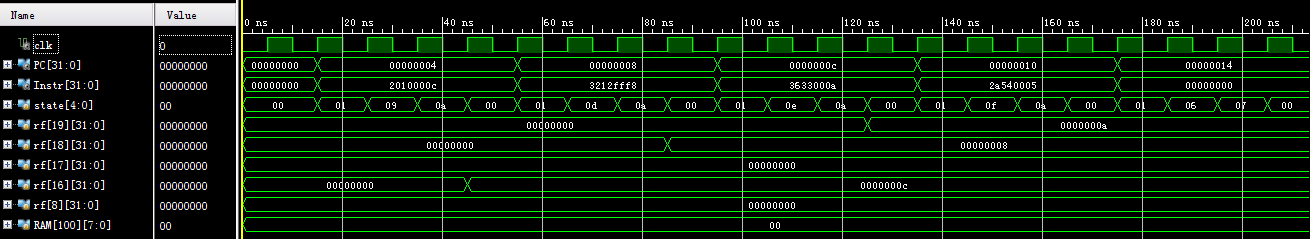
\includegraphics[width =\linewidth]{figure/all1.png}
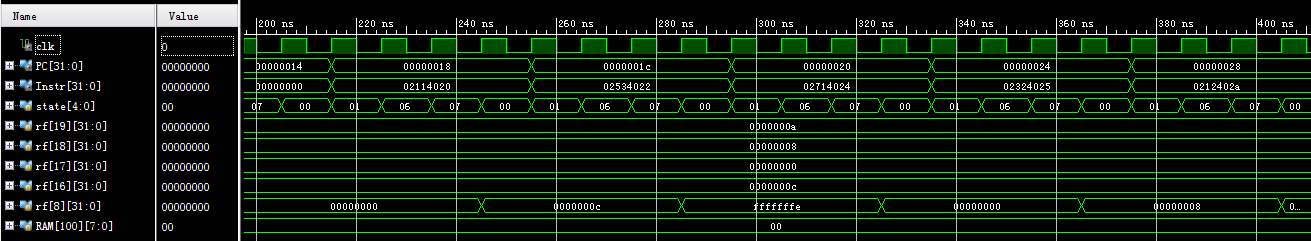
\includegraphics[width =\linewidth]{figure/all2.png}
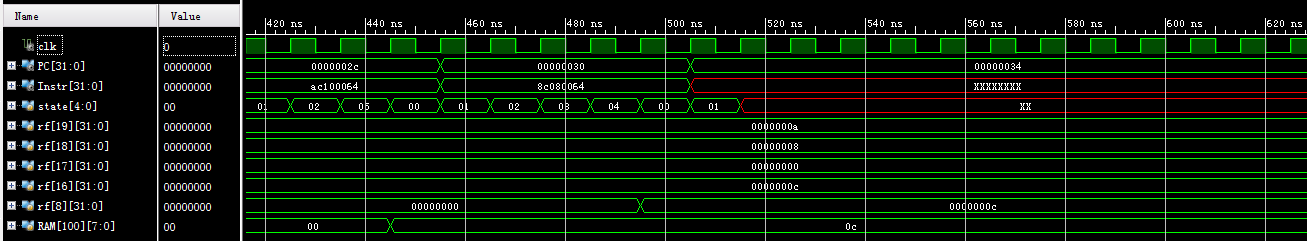
\includegraphics[width =\linewidth]{figure/all3.png}

这里显示了PC、state、instr的值,并可以看到相关变量的运算结果。可以发现,多周期的执行时间明显变长了,而且一条指令会包含多个状态的切换过程。容易验证,所有的运算结果都是正确的。

\subsection{mul.in}

\begin{lstlisting}
 0x0 : addi $s0, $0, 12     | 2010000c
 0x4 : addi $s1, $0, 15     | 2011000f
 0x8 : mul $t0, $s0, $s1    | 72114002
\end{lstlisting}
\noindent
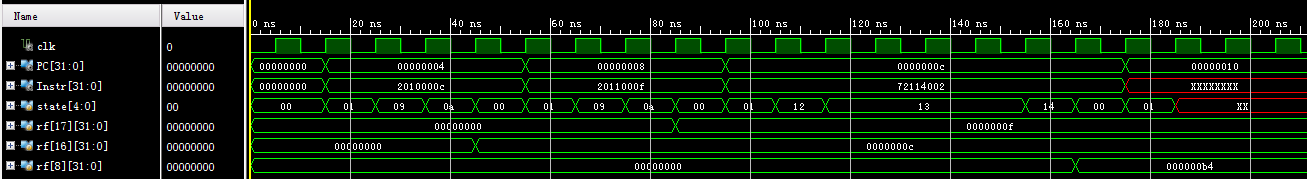
\includegraphics[width =\linewidth]{figure/mul.png}

这一样例简单的演示了乘法的执行过程,首先将s0和s1分别赋值为12和15,然后在用mul运算执行乘法,并把结果写入t0中。可以看到在执行的过程中,状态13的时间是尤其长的,这是因为需要执行四次移位操作。可以看到最后寄存器t0的值为b4=180=12*15,是正确的运算结果。

\subsection{real\_factorial.in}

\begin{lstlisting}
 0x0 : addi $sp, $0, 128    | 201d0080
 0x4 : addi $a0, $0, 4      | 20040004
 0x8 : jal factorial        | 0c000004
 0xc : sll $v0, $v0, 1      | 00021040
0x10 :                      | 
0x10 : factorial:           | 
0x10 : addi $sp, $sp, -8    | 23bdfff8
0x14 : sw $a0, 4($sp)       | afa40004
0x18 : sw $ra, 0($sp)       | afbf0000
0x1c : addi $t0, $0, 2      | 20080002
0x20 : slt $t0, $a0, $t0    | 0088402a
0x24 : beq $t0, $0 ,else    | 10080003
0x28 : addi $v0, $0, 1      | 20020001
0x2c : addi $sp, $sp, 8     | 23bd0008
0x30 : jr $ra               | 03e00008
0x34 : else:                | 
0x34 : addi $a0, $a0, -1    | 2084ffff
0x38 : jal factorial        | 0c000004
0x3c : lw $ra, 0($sp)       | 8fbf0000
0x40 : lw $a0, 4($sp)       | 8fa40004
0x44 : addi $sp, $sp, 8     | 23bd0008
0x48 : mul $v0, $a0, $v0    | 70821002
0x4c : jr $ra               | 03e00008
\end{lstlisting} 
\noindent
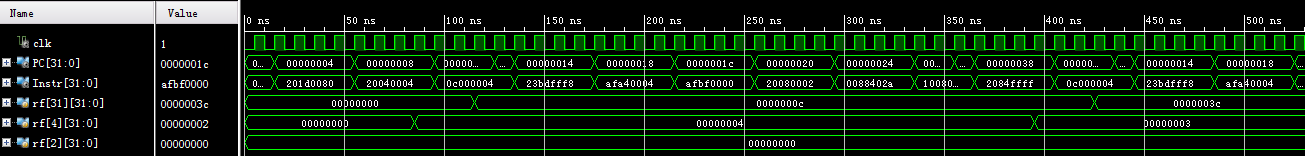
\includegraphics[width =\linewidth]{figure/fac1.png}
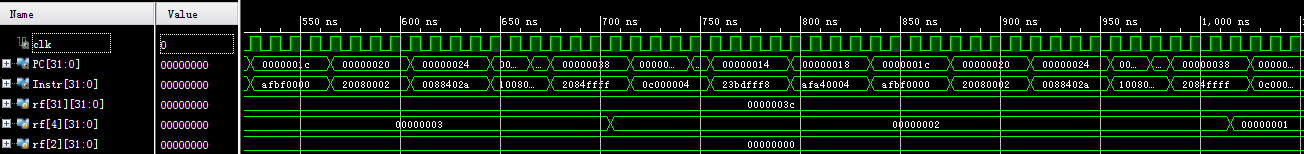
\includegraphics[width =\linewidth]{figure/fac2.png}
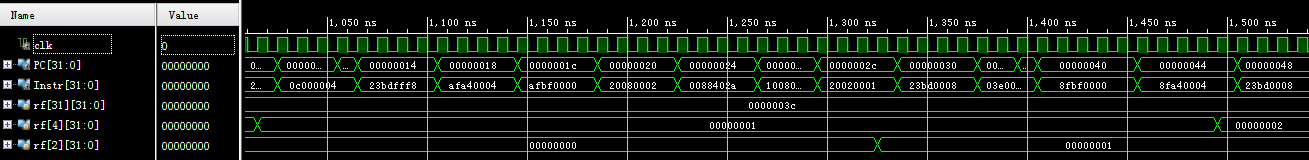
\includegraphics[width =\linewidth]{figure/fac3.png}
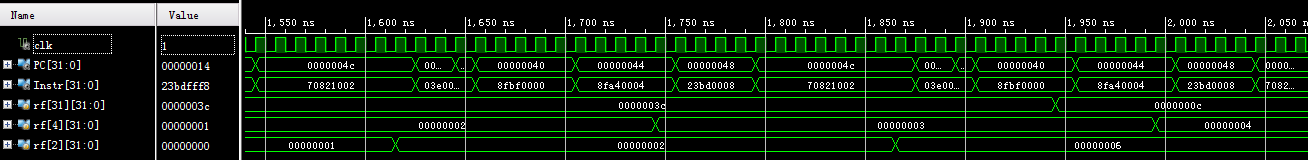
\includegraphics[width =\linewidth]{figure/fac4.png}
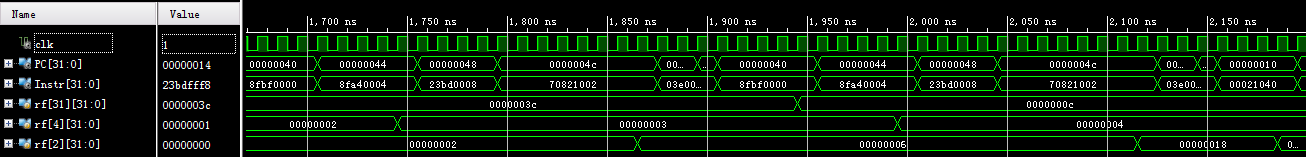
\includegraphics[width =\linewidth]{figure/fac5.png}

因为这幅图耗时略长,所以我把比例调的比较小,以便展示全程。这个样例是递归计算阶乘的小程序,与单周期不同,这次我们实现了乘法器,所以计算的是真正的阶乘。可以看到,ra用于存储返回地址,始终存储的是0xc与0x3c这两个返回地址;a0用于传参,从4逐渐递减至1,又累增至4;v0则用于存储计算结果,初始时一直进行递归调用,所以v0始终保持为0,而后每次v0会与a0相乘,最终得到结果0x18=24=4*3*2*1。另外,可以从PC值看出,程序是正确执行了的。

\section{注意事项}

\subsection{遇到的问题}

想了一下,好像没啥问题。。。

\subsection{显示模块}

这次的显示模块和上次一模一样,不需要做任何改动。不过为了方便演示,我加入了一个暂停功能:
\begin{lstlisting}[language=Verilog]
wire clk, clk0, clk1, clk2, clk3;
clkdiv CLK(CLK100MHZ, clk2, clk1, clk0);
MUX2 #(1) selclk3(sel, clk0, clk1, clk3);
MUX2 #(1) selclk(stop, clk3, 0, clk);
\end{lstlisting}
以sel信号作为调整时钟快慢的信号,以stop信号来控制是否暂停。当stop为1时,直接将0作为时钟信号传入即可。

\section{申A理由}

\begin{itemize}
\item 实现了所有的基本指令
\item 增加了移位指令sll,srl,sra
\item 增加了与函数调用相关的跳转指令jal,jr
\item 增加了乘法指令mul
\item 为乘法指令和函数调用指令添加了相应的测试样例
\end{itemize}

\end{sloppypar}
\end{document}
